\documentclass[10pt,a4paper]{article}
\usepackage[margin=20mm]{geometry}
\usepackage[T1]{fontenc}\usepackage[utf8]{inputenc}
\usepackage{lmodern,microtype,amsmath,amssymb,booktabs,tabularx,graphicx,caption,xcolor,titlesec,fancyhdr,hyperref,xurl}
\setcounter{secnumdepth}{-1}
\definecolor{ink}{HTML}{17252A}\definecolor{teal}{HTML}{176B68}\definecolor{gold}{HTML}{B8892F}
\hypersetup{colorlinks=true,linkcolor=teal,urlcolor=teal,citecolor=teal,pdftitle={Better Than Null Is Not Yet Useful},pdfauthor={Joseph Maxwell}}
\titleformat{\section}{\Large\bfseries\sffamily\color{ink}}{\thesection}{0.6em}{}\titleformat{\subsection}{\large\bfseries\sffamily\color{teal}}{\thesubsection}{0.6em}{}
\captionsetup{font=small,labelfont=bf,justification=raggedright,singlelinecheck=false}
\pagestyle{fancy}\fancyhf{}\fancyhead[L]{\small\sffamily MATERIALS ML FAILURE ANALYSIS}\fancyhead[R]{\small\sffamily FINAL QA V4}\fancyfoot[C]{\small\thepage}\setlength{\headheight}{15pt}
\setlength{\parindent}{0pt}\setlength{\parskip}{5pt plus 1pt}\setlength{\emergencystretch}{2em}
\newcommand{\plainbox}[1]{\begin{center}\fcolorbox{teal}{teal!5}{\begin{minipage}{0.92\linewidth}#1\end{minipage}}\end{center}}
\title{Better Than Null Is Not Yet Useful\\\large Failure Analysis of Model Viability in Materials Informatics}
\author{Joseph Maxwell\\\small The Systemica Institute, London, United Kingdom\\\small ORCID: \href{https://orcid.org/0009-0002-4070-6035}{0009-0002-4070-6035}\\\small \href{mailto:j.maxwell@systemicainstitute.org}{j.maxwell@systemicainstitute.org}}
\date{Preprint -- August 2026}
\begin{document}\maketitle

\begin{abstract}
A target-permutation null asks whether a model learned more than a deliberately broken training route. Absolute predictive performance asks whether the model improves on a task-relevant constant reference. These questions can disagree. We examined a frozen Materials Project elasticity audit using the same 288 baseline cells for both judgements. Of these cells, 211 (73.3\%) had positive separation from their paired permutation null. Only 13 (4.51\%) had positive held-out $R^2$, and the same 13 passed both conditions. All conjunctive passes were bulk-modulus cells. Across the wider 1,152-cell elastic route, only 20 cells (1.74\%) had positive $R^2$, and median $R^2$ was $-2.248$. The models had often learned more than the permuted-target comparator while still performing worse than the constant evaluated-set mean-target reference. We therefore retain non-null signal and absolute predictive viability as separate gates and require both for the demonstrated route. Here, $R^2>0$ is only the lowest boundary against that constant reference; it is not a universal engineering threshold. Source admission remains a separate scientific question. The result is a failure analysis of one bounded materials workflow, not experimental qualification or a universal acceptance rule.
\end{abstract}

\plainbox{\textbf{This paper in plain language}\par
\textbf{Question:} If a model performs better than deliberately broken versions of itself, does that mean it predicts well enough to be useful?\par
\textbf{Why it matters:} ``Better than broken labels'' and ``clears an absolute predictive boundary'' are different claims.\par
\textbf{What we did:} We compared valid Materials Project elasticity models with matched shuffled-target controls, then checked held-out $R^2$.\par
\textbf{What we found:} On the same 288 cases, \textbf{73.3\% beat the null but only 4.51\% had positive $R^2$}.\par
\textbf{What it does not mean:} $R^2>0$ is only a minimal metric reference, not an engineering deployment threshold.}

\noindent\textbf{Three ways to read this paper.} \textbf{Just want the answer?} Read the box, Figure~\ref{fig:same}, and the Conclusion. \textbf{Want the experiment?} Read Materials and Methods plus Results. \textbf{Want to audit it?} Follow the public scientific-method specification, accepted evidence, and reconstruction package.

\section{1. Introduction}
A target-permutation test breaks the relation between the training inputs and targets. If a valid model outperforms models trained on those shuffled targets, it has detected target-linked structure that the broken route does not retain.

That comparison is relative. It does not establish that the resulting predictor is useful in absolute terms. A model can outperform a random-number generator and still be a poor thermometer.

For regression, $R^2$ provides one minimal reference. Positive held-out $R^2$ means the model reduces squared error relative to predicting the mean of the evaluated targets. Negative $R^2$ means the constant reference performs better. This boundary is weak compared with most engineering requirements, but it is sufficient to reveal a basic contradiction.

We asked: \emph{can a materials model beat a paired target-permutation null and still fail even this minimal absolute predictive baseline?}

The answer was measured on the same 288 Materials Project elasticity cells. Positive null separation occurred in 211 cells. Positive $R^2$ occurred in only 13. The same 13 passed both tests. Thus, 198 cells carried relative-only signal.

This paper contributes three things. It measures the divergence on a common denominator. It records the two outcomes conjunctively rather than averaging them. It also shows why source admission and model viability must remain orthogonal: a scientifically admissible target may be poorly modelled, and a statistically promising route may still depend on unresolved source semantics.

The contribution is not the algebraic observation that relative and absolute inequalities differ. It is the empirical failure analysis showing that this distinction affected most eligible cells in a frozen materials workflow, and the resulting separation of those measurements in reporting and adjudication.

\section{2. Materials and Methods}
\subsection{2.1 Materials Project source and elastic route}
The source was a checkpointed Materials Project API snapshot acquired on 28 July 2026 and bound by SHA-256. The source universe contained approximately 154,377 records; 154,373 entered the processed maximum-coverage routes. Elastic maximum-coverage cohorts contained 13,028 records for bulk and shear modulus. The stricter four-target common cohort contained 13,021.

Each elastic target was evaluated in two cohorts and two descriptor lanes. The common lane contained 11 descriptors: density, volume per atom, number of sites, total magnetisation, six lattice parameters, and crystal system. The target-specific lane added formation energy per atom, energy above hull, stability flag, band gap, and metallicity, giving 16 descriptors. Target and proxy exclusions were checked before fitting.

\subsection{2.2 Models, preprocessing, and hyperparameters}
All four models used the same scikit-learn 1.8.0 preprocessing. Numeric fields received median imputation followed by standardisation. Crystal system received most-frequent imputation and dense one-hot encoding with unknown categories ignored. Every transformer was fit on the training partition only. No target transform was applied.

\begin{table}[htbp]\centering\small
\caption{Frozen model settings. Parameters not shown as explicit used the constructor defaults of the bound scikit-learn 1.8.0 environment; the method supplement records those defaults.}
\begin{tabularx}{\linewidth}{@{}p{0.22\linewidth}X@{}}\toprule
Model & Frozen settings\\\midrule
Ridge & $\alpha=1.0$; intercept fitted; automatic solver; tolerance $10^{-4}$\\
Random forest & 200 trees; minimum leaf size 2; all features considered at a split; squared-error criterion; no depth limit; bootstrap sampling; \texttt{random\_state=seed}\\
Extra Trees & 300 trees; minimum leaf size 2; all features considered at a split; squared-error criterion; no depth limit; no bootstrap; \texttt{random\_state=seed}\\
Histogram gradient boosting & 250 boosting iterations; depth 6; learning rate 0.05; squared-error loss; minimum leaf size 20; no L2 penalty; automatic early stopping; \texttt{random\_state=seed}\\\bottomrule
\end{tabularx}\end{table}

The three seeds were 11, 23, and 37. Tree ensembles used all available local cores inside each scientific subprocess, as specified by \texttt{n\_jobs=-1}.

\subsection{2.3 Population splits and scale design}
Three deterministic 80/20 split views were used. The row-random view hashed the record identifier. The composition-group view hashed a reduced-composition identifier. The chemical-system view hashed the chemical-system identifier. For each view and seed, a SHA-256-derived bucket below 2,000 of 10,000 assigned the complete group to test; all other buckets assigned it to train. No stratification was applied.

The route evaluated 2,000, 5,000, 10,000, and full-cohort scales. Subsets were selected by a deterministic hash order of record identifiers. If a cohort was smaller than a requested scale, the complete cohort was used.

\subsection{2.4 Target-permutation null}
Paired nulls were calculated at full scale. For each eligible valid cell, the paired null estimate was the mean $R^2$ across 30 otherwise matched target-permutation refits. In each refit, the training targets were shuffled. Permutation repetition $r$ used random state $1000s+r$, where $s$ was the model seed. Inputs, preprocessing, model family, split membership, held-out targets, and hyperparameters remained unchanged. Each null model was refitted from the beginning.

We define relative separation as
\[
S_{R^2}=R^2_{\mathrm{valid}}-\overline{R^2_{\mathrm{permuted}}}.
\]
Positive $S_{R^2}$ indicates that the valid route outperformed its paired broken-target route.

\subsection{2.5 Metrics and same-denominator eligibility}
Predictions were evaluated with \texttt{sklearn.metrics.r2\_score} and mean absolute error. For an evaluated test vector $y$,
\[
R^2=1-\frac{\sum_i(y_i-\hat y_i)^2}{\sum_i(y_i-\bar y_{\mathrm{test}})^2}.
\]
The denominator therefore uses the mean of the evaluated held-out targets, not the training-target mean.

The complete elastic route contained
\[
2\ \mathrm{targets}\times2\ \mathrm{cohorts}\times2\ \mathrm{lanes}\times4\ \mathrm{scales}\times3\ \mathrm{splits}\times3\ \mathrm{seeds}\times4\ \mathrm{models}=1{,}152
\]
baseline cells. Paired nulls existed only at full scale. Restricting to cells with non-missing baseline $R^2$, mean null $R^2$, and $S_{R^2}$ produced
\[
2\times2\times2\times1\times3\times3\times4=288
\]
null-comparable cells. The 73.3\%, 4.51\%, and conjunctive 4.51\% results all use these same 288 cells.

\textbf{Model-evaluation cell:} one target $\times$ cohort $\times$ descriptor lane $\times$ scale $\times$ split $\times$ seed $\times$ model configuration. It is one declared comparison case, not necessarily one model fit.

A cell is an analysis coordinate, whereas a scientific unit is a contract-bound execution boundary. A unit can contain more than one estimator fit. For example, the earlier Matbench null route contained 20 official-fold units, each with one baseline fit and five target-permutation refits: 20 scientific units represented 120 estimator fits. The public scale register therefore keeps cells, units, and fits separate.

The $R^2>0$ boundary compares squared error with the constant evaluated-set reference inherent to the metric. It is not presented as a deployable predictor, application-specific engineering baseline, or sufficient condition for practical usefulness.

\subsection{2.6 Replay and evidence extraction}
The scientific programme comprised 64 fresh and 64 replay units. The replay comparator examined 37,924 numeric cells with an absolute tolerance of $10^{-10}$. It retained 916 strict exceedances, all in elastic routes. The replay is therefore not described as exact for elasticity.

The 288-cell table used here was extracted read-only from the sealed fresh payload. No model was refitted for this paper. The replay exceedances do not alter the reported fresh-payload same-denominator counts; they instead bound the repeatability claim for the elastic route.

\section{3. Results}
\subsection{3.1 The same 288 cells gave different conclusions}
Among the 288 paired-null-comparable elastic cells, 211 (73.3\%) had $S_{R^2}>0$. Only 13 (4.51\%) had $R^2>0$. Those same 13 passed both conditions (Figure~\ref{fig:same}). Thus, beating the paired null was common, whereas beating the constant mean-target reference was rare.

\begin{figure}[htbp]\centering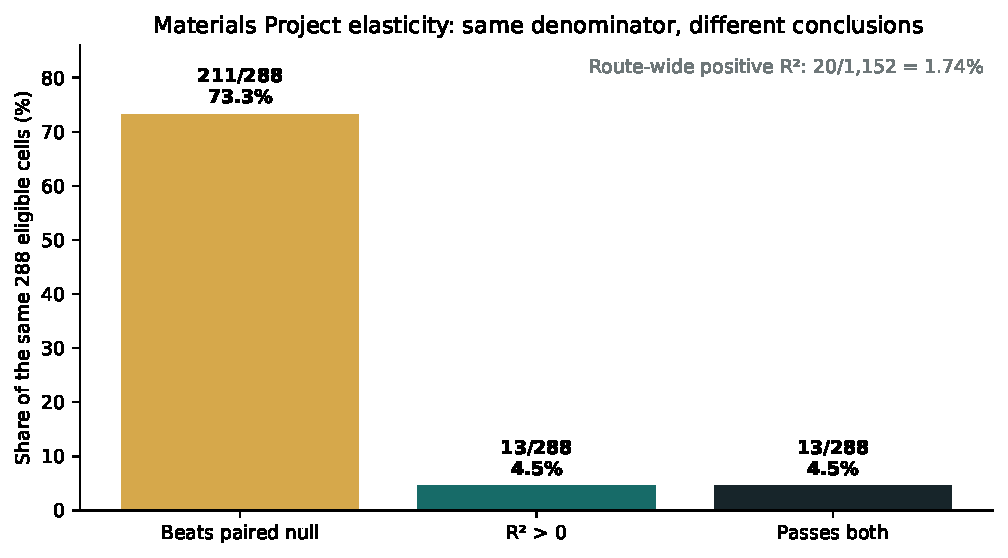
\includegraphics[width=0.78\linewidth]{figures/PAPER_2_MP_SAME_DENOMINATOR.pdf}\caption{\textbf{Most models beat their broken-target controls, but almost none cleared the minimal absolute $R^2$ boundary.} The relative and absolute results use the same 288 model-evaluation cells.}\label{fig:same}\end{figure}

\subsection{3.2 Bulk and shear breakdown}
Bulk and shear each contributed 144 null-comparable cells. Positive null separation occurred in 79.9\% of bulk cells and 66.7\% of shear cells. All 13 conjunctive passes were bulk cells. Shear contributed none.

Across all scales, bulk had median $R^2=-4.866$ and 3.13\% positive $R^2$. Shear had median $R^2=-0.688$ and 0.35\% positive $R^2$. Both targets therefore displayed the same qualitative failure despite different distributions.

\subsection{3.3 Route-wide absolute performance}
Across all 1,152 elastic baseline cells, only 20 (1.74\%) had positive $R^2$. Median $R^2$ was $-2.248117$. The negative median means that more than half of the evaluated routes performed worse than the constant mean-target reference. Extreme negative values were retained rather than clipped or averaged away.

\subsection{3.4 Historical context}
An earlier report-bound adjudication found positive separation in approximately 88\% of raw elastic model cells while median $R^2$ remained negative. That observation motivated this failure analysis. It used a different admissible boundary and is not interchangeable with the machine-readable 211/288 result. The same-denominator extraction is the primary evidence in this paper.

\subsection{3.5 Replay result}
The fresh and replay routes each completed 64 units. Of 37,924 compared numeric cells, 916 exceeded the strict $10^{-10}$ tolerance, all in elastic outputs. This adverse replay state is part of the result. It prevents the elastic route from being described as an exact numerical replay.

\section{4. Interpretation: Two Independent Gates}
The failure requires two independently inspectable questions (Figure~\ref{fig:gate}).

\textbf{Gate A: non-null signal.} Does the valid route outperform its paired target-permutation null, so that $S_{R^2}>0$?

\textbf{Gate B: absolute viability.} Does the valid route exceed the declared absolute task boundary? For this demonstration only, the minimal boundary is $R^2>0$.

The route passes the demonstrated screen only when both gates pass. Positive null separation cannot repair negative absolute performance. Positive $R^2$ without positive null separation would also require scrutiny because the result would not exceed the paired broken-target route.

\begin{figure}[htbp]\centering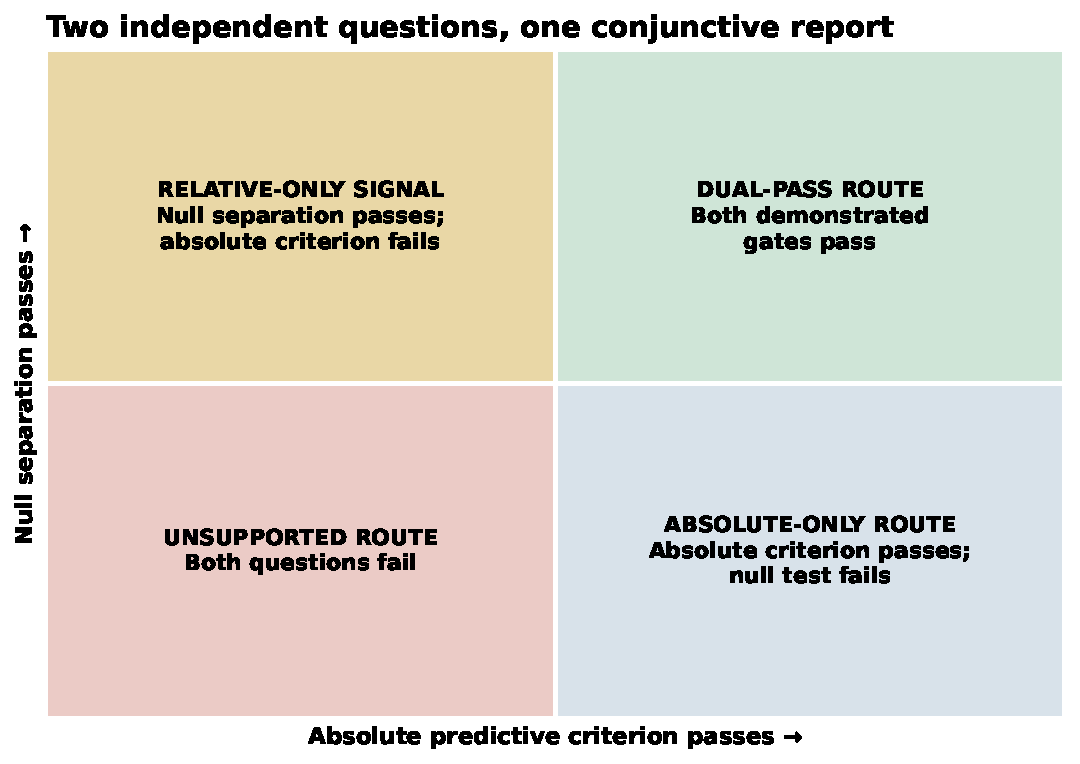
\includegraphics[width=0.78\linewidth]{figures/PAPER_2_TWO_GATE_MAP_REVIEWER_HARDENED.pdf}\caption{\textbf{Relative signal and absolute prediction remain separate decisions.} Conjunctive reporting preserves four possible states. ``Dual-pass'' means only that both demonstrated gates pass; it does not imply deployment readiness or engineering usefulness.}\label{fig:gate}\end{figure}

This is not a proposal that $R^2>0$ is sufficient for engineering use. It is the lowest demonstrated boundary against the constant evaluated-set mean-target reference. Real decisions may require substantially stronger error, uncertainty, ranking, domain, and consequence thresholds.

\section{5. Supporting Diagnostics}
\subsection{5.1 Source admission is orthogonal}
A prospective no-fit audit assessed 26,056 Materials Project elastic record-target pairs. It classified 23,891 as conditional and 2,165 as anomalous or unresolved. None reached the strongest category under the predeclared admission rubric used in this study because tensor-level and method evidence were incomplete. This does not mean those records are corrupt. It means source availability did not establish the strongest admissibility status.

Source admission and model viability are independent. An admissible target may still be poorly represented by a model. A statistically viable model may still rest on unresolved property semantics.

\subsection{5.2 Bounded comparators}
Separate JARVIS routes showed that positive held-out $R^2$ and null separation can coexist under this broader experimental design. Curated Matbench tasks also supplied substantial positive held-out predictive performance. A 256-material spatial confirmation provided another conjunctive example: bulk metric geometry passed two required population views, whereas shear polarity passed one and failed the other. None of these comparators changes the Materials Project result; they show that the gate can return different bounded outcomes.

\section{6. Engineering Implications}
Materials models can influence which candidates advance to higher-fidelity simulation, synthesis, microscopy, or mechanical testing. A route that merely beats a deliberately broken comparator has not earned those actions. In this case, 198 of the 288 comparable cells would have passed on null separation alone despite failing the $R^2>0$ boundary.

The present work did not execute or validate an industrial materials decision. Its engineering contribution is a bounded warning: relative success should not be allowed to substitute for task-appropriate predictive adequacy.

\section{7. Limitations and Falsification}
The result concerns one Materials Project snapshot, a compact descriptor representation, four classical model families, three split views, three seeds, and the declared cohort design. Elastic source semantics remained unresolved at the strongest level. The 916 replay exceedances require continued implementation and source scrutiny. The extreme negative $R^2$ tail may reflect multiple causes, including difficult targets, inadequate representation, source anomalies, grouping, and model behaviour; this study does not uniquely assign cause.

Future falsification should use tensor- and method-resolved elastic cohorts, prospectively frozen admission rules, alternative representations, and application-specific viability thresholds. Higher-fidelity graph or atomistic models should be added only under a separate protocol. Physical qualification would require independent calculation or experiment.

\section{8. Conclusion}
A materials model can beat a paired target-permutation null and still fail a minimal absolute baseline. On the same 288 Materials Project elastic cells, 73.3\% beat their paired null, but only 4.51\% achieved positive $R^2$. The same 4.51\% passed both conditions.

The methodological consequence is simple: non-null signal and absolute predictive viability must be reported separately and passed conjunctively when both are required. Beating a broken comparator is evidence of signal. It is not, by itself, evidence of usefulness.

\textbf{If you remember one thing:} beating a broken comparator establishes relative signal, not absolute predictive usefulness.

\section*{Declarations}
\textbf{Funding.} This research was conducted independently without dedicated external research grant funding.

\textbf{Competing interests.} The author is founder of a venture developing software and services related to scientific evidence assurance and engineering decision support described in this work.

\textbf{AI assistance.} AI and coding tools assisted code development, critique, diagnosis, evidence organisation, and manuscript preparation. They did not generate source target data. Frozen analyses were executed by conventional scientific software under declared protocols, and scientific interpretations and conclusions were reviewed by the author.

\textbf{Data and code availability.} A public research compendium contains accepted derived evidence and publication-specific reconstruction code. The exact scientific configuration is also provided as a paper-specific method record. Raw provider datasets remain subject to their source terms.

\section*{References}\small
\begin{enumerate}
\item Ojala, M. and Garriga, G. C. Permutation tests for studying classifier performance. \emph{JMLR} 11, 1833--1863 (2010).
\item Jain, A. et al. The Materials Project: a materials genome approach to accelerating materials innovation. \emph{APL Materials} 1, 011002 (2013).
\item Dunn, A. et al. Benchmarking materials property prediction methods: the Matbench test set and Automatminer reference algorithm. \emph{npj Computational Materials} 6, 138 (2020).
\item Choudhary, K. et al. The joint automated repository for various integrated simulations (JARVIS) for data-driven materials design. \emph{npj Computational Materials} 6, 173 (2020).
\item Li, K. et al. Generalization error of machine learning interatomic potentials and the importance of out-of-distribution assessment. \emph{npj Computational Materials} (2024).
\item Tran, K. et al. Methods for comparing uncertainty quantifications for material property predictions. \emph{Machine Learning: Science and Technology} 1, 025006 (2020).
\end{enumerate}
\end{document}
